\documentclass[10pt,a4paper]{book}

\usepackage[utf8]{inputenc}
\usepackage[T1]{fontenc}
\usepackage[french]{babel}
%\renewcommand\sfdefault{phv}
\usepackage[left=2cm, right=2cm, bottom=1.85cm, top=1.5cm]{geometry}

\usepackage{fancyhdr}
\usepackage{framed}
\pagestyle{fancy}
\usepackage{hyperref}
%\renewcommand{\headrulewidth}{1pt}
%\fancyhead[C]{\textbf{page \thepage}} 
\fancyhead[L]{Cours}
\fancyhead[R]{Seconde}
\usepackage[skip=15pt plus1pt, indent=15pt]{parskip}

\renewcommand{\footrulewidth}{1pt}
\fancyfoot[C]{\textbf{page \thepage}} 
\fancyfoot[L]{Lycée Jacques Brel}
\fancyfoot[R]{Année 2022-2023}

%%%%%%%%%%%%%%%%%%%%%%%%%%%%%%%%%%%%%%%%%%%%%%%%%%

%\newcommand{\TDoc}[1]{
%\begin{center}
%{\setlength{\fboxsep}{10pt}  % Ecart texte-boite
%\shadowbox{\textbf{\Large{#1}}}}
%\end{center}
%\vspace{1.5cm}}
    
 \usepackage{fancybox}   %pour l'encadré du titre shadowbox
 \usepackage{stmaryrd}   %pour utiliser correctement les crochets pour les ensembles de définitions
 \usepackage[normalem]{ulem}
 \usepackage{graphicx}
 %\usepackage{wrapfig} %texte coulé autour d'une image
 \usepackage{soul} % souligné
 \usepackage{nonfloat}
 \usepackage[standard]{ntheorem}
 \usepackage{array}
 \usepackage{arydshln}
 \usepackage{graphicx}
%MATHEMATIQUES
\usepackage{amsmath,amsfonts} 

\usepackage{tikz}
\newcommand{\N}{\mathbb{N}}
\newcommand{\Z}{\mathbb{Z}}
\newcommand{\D}{\mathbb{D}}
\newcommand{\Q}{\mathbb{Q}}
\newcommand{\R}{\mathbb{R}}
\newcommand{\Co}{\mathbb{C}}
\newcommand{\K}{\mathbb{K}}
\newcommand{\F}{\mathbb{F}}


%%%%%%%%%%%%%%%%%%%%%%%%%%%%%%%%%%%

\makeatletter
%%%%%%%%%%%%%%%%%%% debut fichier boiboites.sty %%%%%%%%%%%%%%%%%%%%%%
\RequirePackage{xkeyval}
\RequirePackage{tikz}
\usetikzlibrary{intersections}
\usetikzlibrary{positioning}
\usetikzlibrary{3d}
\RequirePackage{amssymb}

\define@key{boxedtheorem}{titlecolor}{\def\titlecolor{#1}}
\define@key{boxedtheorem}{titlebackground}{\def\titlebackground{#1}}
\define@key{boxedtheorem}{background}{\def\background{#1}}
\define@key{boxedtheorem}{titleboxcolor}{\def\titleboxcolor{#1}}
\define@key{boxedtheorem}{boxcolor}{\def\boxcolor{#1}}
\define@key{boxedtheorem}{thcounter}{\def\thcounter{#1}}
\define@key{boxedtheorem}{size}{\def\size{#1}}
\presetkeys{boxedtheorem}{titlecolor = black, titlebackground = white, background = white,%
                         titleboxcolor = black, boxcolor = black, thcounter=, size = .9\textwidth}{}

\newcommand{\couleurs}[1][]{%
    \setkeys{boxedtheorem}{#1}
    \tikzstyle{fancytitle} =[draw=\titleboxcolor, rounded corners, fill=\titlebackground,
                            text= \titlecolor]
    \tikzstyle{mybox} = [draw=\boxcolor, fill=\background, very thick,
                        rectangle, rounded corners, inner sep=10pt, inner ysep=20pt]
}


%Commande generique pour faire un joli encadre
\newsavebox{\boiboite}
\newcommand{\titre}{Titre}
\newenvironment{boite}[2][]%
    {%
    \renewcommand{\titre}{#2}
    \couleurs[#1]
    \begin{lrbox}{\boiboite}%
     \begin{minipage}[!h]{\size}
    }%
    {%
     \end{minipage}
    \end{lrbox}
    \begin{center}
    \begin{tikzpicture}
    \node [mybox] (box){\usebox{\boiboite}};
    \node[fancytitle, right=10pt] at (box.north west) {\titre};
    \end{tikzpicture}
    \end{center}
    }

\newcommand{\newboxedtheorem}[4][]{%
    \couleurs[#1]
    \@ifnotempty{#4}{%
      \@ifundefined{the#4}{\@ifundefined{\thcounter}{\newcounter{#4}}{%
      \newcounter{#4}[\thcounter ] } } { }%
    }
    \newenvironment{#2}[1][]{%
    \@ifnotempty{#4}{\refstepcounter{#4}}
    \begin{boite}[#1]{\textbf{#3\@ifnotempty{#4}{ \csname the#4\endcsname}}\@ifnotempty{##1}{
    (##1)}}
    }%
    {%
    \end{boite}
    }
}

\newcommand{\newboxedtheoreme}[4][]{%
    \couleurs[#1]
    \@ifnotempty{#4}{%
      \@ifundefined{the#4}{\@ifundefined{}{}{%
      } } { }%
    }
    \newenvironment{#2}[1][]{%
    \@ifnotempty{#4}{\refstepcounter{#4}}
    \begin{boite}[#1]{\textbf{#3\@ifnotempty{#4}{ \csname the#4\endcsname}}\@ifnotempty{##1}{
    (##1)}}
    }%
    {%
    \end{boite}
    }
}
%%%%%%%%%%%%%%%%%%%% end fichier boiboites.sty %%%%%%%%%%%%%%%%%%%%%%


\newboxedtheorem{theo}{Théorème}{theorem}
\newboxedtheorem{de}{D\'efinition}{theorem}
\newboxedtheorem{prop}{Propriété}{theorem}
\newboxedtheorem{pro}{Proposition}{theorem}
\newboxedtheorem{nota}{Notation}{theorem}
\newboxedtheorem{act}{Activité}{theorem}
\newtheorem{exo}{Exercice}
\newboxedtheorem{exe}{Exemple}{theorem}
\newboxedtheorem{cor}{Corolaire}{theorem}
\newboxedtheoreme{conc}{Conclusion}{theorem*}
\newboxedtheoreme{demo}{\textbf{Démonstration guidée}}{theorem}
%%%%%%%%%%%%%%%%%%%%%%%%%%%%%%
%%%%%%%%%%%%%%%%%%%%%%%%%%%%%
\newlength{\longA}
\newlength{\longB}
\newenvironment{BoiteShadow}[3][\linewidth]{%
\addtolength{\longA}{#2}
\addtolength{\longB}{#3}
\begin{Sbox}\begin{minipage}{#1}}%
{\end{minipage}\end{Sbox}%
\setlength{\fboxsep}{\longA}
\setlength{\shadowsize}{\longB}
\shadowbox{\unhbox\@Sbox}\par}
\makeatother
\author{Augustin WENGER}

\title{Cours SNT Seconde 1 2022-2023}
\date{\today}

%%%% fin du préambule, on passe au contenu : tout le texte entre
%%%% \begin{document} et \end{document} 

\begin{document}
\maketitle
\tableofcontents
\chapter{Codage d'informations sur un ordinateur}


Ce chapitre d'introduction présente rapidement les différentes manières de stocker des données sur un ordinateur.

\section{Structure d'un disque dur}

Un disque dur d'ordinateur est constitué d'un grand nombre de cellules magnétiques dont chacune contient une information binaire : si une cellule est aimantée dans un certain sens, on considère qu'elle contient un 1, sinon on considère qu'elle contient un 0.

Un disque dur dispose de têtes de lecture, qui sont capables de mesurer la charge magnétique d'une cellule pour voir si elle contient un 1 ou un 0, ainsi que de têtes d'écriture, qui sont capables de modifier la charge magnétique d'une cellule en fonction des informations à inscrire dans le disque dur.


\subsection{Combien d'informations peut-on stocker dans un disque dur ?}

Un disque dur est donc comme un grand livre, dont chaque caractère serait constitué uniquement des lettres "1" et "0". On se demande combien il y a de manières d'écrire ce livre en fonction du nombre de cellules du disque dur.

\begin{act}
    Vous disposez de 3 jetons qui sont blanc d'un côté et noir de l'autre. Pour transmettre un message à un camarade qui est sorti de la pièce, vous devez les placer dans 3 cases, sur la face de votre choix. Combien de messages différents pouvez vous envoyer ?
\end{act}


Prenons l'exemple d'un disque dur ayant 3 cellules. Il y a exactement $2^3=8$ mots de $3$ lettres constitués exclusivement des lettres "0" et "1":

\begin{center}
    \begin{tabular}{|c|c|}
         \hline
         000 & 100  \\
         \hline
         001 & 101 \\
         \hline
         010 & 110 \\
         \hline
         011 & 111\\
         \hline
    \end{tabular}
\end{center}

Pour chacune des cellules, il y a 2 possibilités différentes. Plus généralement, s'il y a $n$ cellules le nombre de messages différents qui peut être stocké dans un ordinateur est donc de $2^{n}$.

On voit que le nombre de cellules est le paramètre qui permet de déterminer le nombre de messages différents qui peuvent être codés. On appelle le nombre de cellules le nombre de \textbf{bits} du disque dur.



\subsection{Comment parle-t-on de la quantité de mémoire d'un ordinateur ?}


\begin{de}
Pour décrire la mémoire d'un ordinateur, on parle plus souvent en \textbf{octets} qu'en bits. Un octet représente 8 cellules. On utilise donc la formule de conversion suivante :
\begin{center}
    $1$ octet = $8$ bits
\end{center}
\end{de}

De plus, il y a énormément de cellules dans un ordinateur. Pour compter le nombre d'octets, on utilise les préfixes classiques multiplicateurs :

\begin{center}
    \begin{tabular}{|c|c|c|}
         \hline
         préfixe &  quantité &  puissance de 10 \\
         \hline
         kilo- & 1 000 & $10^3$ \\
         \hline
         mega- & 1 000 000 & $10^6$ \\
         \hline
         giga- & 1 000 000 000 & $10^9$ \\
         \hline
         tera- & 1 000 000 000 000 & $10^{12}$ \\
         \hline
         peta- & 1 000 000 000 000 000 & $10^{15}$ \\
         \hline
    \end{tabular}
\end{center}

Et l'on obtient le tableau suivant

\begin{center}
    \begin{tabular}{|c|c|c|c|}
         \hline
         nom & symbole  &nombre d'octets &  nombre de bits \\
         \hline
         kilooctet & Ko &1 000 octets & 8 000 bits \\
         \hline
         megaoctet & Mo & 1 000 000 octets& 8 000 000 000bits  \\
         \hline
         gigaoctet & Go & 1 000 000 000 octets&  8 000 000 000 bits  \\
         \hline
         teraoctet & To & 1 000 000 000 000 octets&  8 000 000 000 000 bits  \\
         \hline
         petaoctet & Po & 1 000 000 000 000 000 octets&  8 000 000 000 000 000 bits  \\
         \hline
    \end{tabular}
\end{center}

Par exemple, un disque dur de 50 Go fait 50 Gigaoctets, donc 50 milliard d'octets donc 400 milliards de cellules. 



\section{Stocker des informations}

On dispose maintenant d'un disque dur qui sait stocker des grandes quantités d'informations et y accéder. Une autre étape nécessaire est celle de coder les informations sous la forme binaire.

La manière dont toute information est codée dépend du format du fichier. On va voir quelques exemples :

\section{Stocker du texte}

Pour stocker du texte dans un disque dur, il faut inventer un codage : un algorithme de transformation qui permette de transformer un texte en une série de 0 et de 1, et inversement.

\begin{de}
Un \underline{algorithme} est une suite d'instructions détaillées qui, si elles sont correctement exécutées, conduit à un résultat donné. 
\end{de}

Le côté inversible de l'opération est très important : pour pouvoir récupérer les informations présentes dans le disque dur, il faut que l'on puisse repasser de l'écriture binaire à une écriture sous la forme de texte.

Essayons de fabriquer un dictionnaire qui code chaque lettre sous la forme d'un mot constitué de 0 et de 1. 


\subsection{Une méthode qui ne marche pas : utiliser le code Morse}

Une approche naïve consisterait à prendre un alphabet existant qui ne contient que deux lettres différentes, par exemple l'alphabet morse ( cf Figure ~\ref{fig:Ensembles})

\begin{figure}[htbp]
\centering
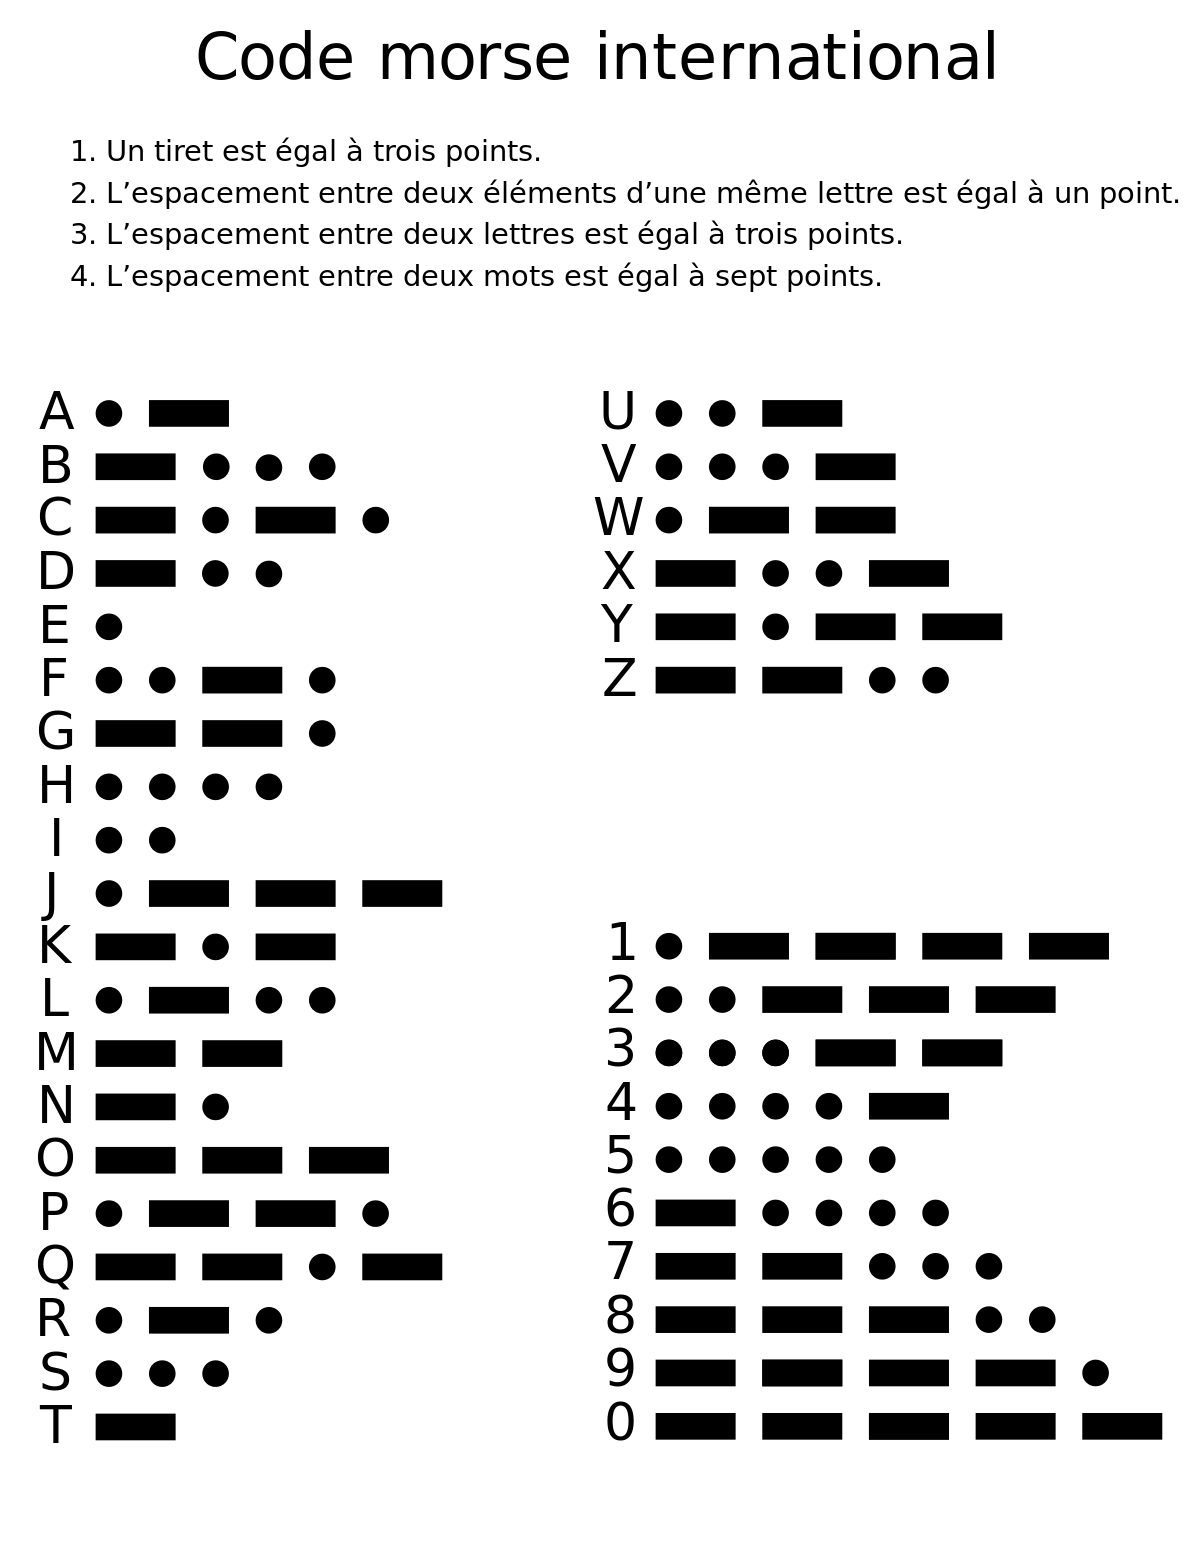
\includegraphics[width=0.5\textwidth]{morse.png}
\caption{L'alphabet morse}
\label{fig:Ensembles}
\end{figure}


On pourrait rêver de transformer cet alphabet en binaire, par exemple en remplaçant les points par des 0 et les traits par des 1.  Par exemple, pour coder le mot CHIEN :


\begin{center}
    \begin{tabular}{|c|c|c|c|c|c|}
         \hline
         Mot & C & H & I & E & N \\
         \hline
         Morse & -.-. & .... & .. & . & -.  \\
         \hline
         Binaire & 1010 & 0000 & 00 & 0 & 10\\
         \hline
         Codage final &\multicolumn{5}{c|}{1010000000010}\\
         \hline
    \end{tabular}
\end{center}

Le mot CHIEN s'écrirait donc dans l'ordinateur comme 1010000000010

Mais on se rend compte que cela ne suffira pas : Quand on communique en morse, on laisse des temps plus longs entre les lettres, mais on ne pourra pas faire la même chose en binaire. par exemple, si on essaye de traduire les mots BASE et DITES, on s'aperçoit qu'ils s'écriraient pareil.



\begin{center}
\begin {tabular}{cc}
    \begin{tabular}{|c|c|c|c|c|c|}
         \hline
         Mot & D & I & T & E & S \\
         \hline
         Morse &-.. & .. & - & . & ...\\
         \hline
         Binaire & 100 & 00 & 1 & 0 & 000\\
         \hline
         Codage final &\multicolumn{5}{c|}{1000010000}\\
         \hline
    \end{tabular}

    \begin{tabular}{|c|c|c|c|c|}
         \hline
         Mot & B & A & S & E \\
         \hline
         Morse & -... & .- & ... & .\\
         \hline
         Binaire & 1000 & 01 & 000 & 0\\
         \hline
         Codage final &\multicolumn{4}{c|}{1000010000}\\
         \hline
    \end{tabular}
\end{tabular}

\end{center}

Le problème, c'est qu'on a bien une liste de lettres qui sont uniquement identifiées, mais comme on ne sait pas quand on a fini d'écrire une lettre, on ne peut pas décoder le code obtenu.

\subsection{Plusieurs moyens de résoudre ce problème}

On peut essayer d'imaginer plusieurs techniques pour passer outre ce problème :
\begin{itemize}
    \item Faire en sorte que chaque lettre possède le même nombre de caractères binaires. Par exemple, si une lettre est codée sur 8 bits (un octet), on sépare les données en groupes de 8 bits et l'on récupèrera les lettres. Par exemple, pour un alphabet à 4 lettres, on aurait (en codant chaque lettre sur 2 bits):
        \begin{center}
            \begin {tabular}{|c|c|}
                     \hline
                \item Lettre & Code \\
                     \hline
                \item A & 00\\
                     \hline
                \item B & 01\\
                     \hline
                \item C & 10\\
                     \hline
                \item D & 11\\
                     \hline
            \end{tabular}
        \end{center}
    \item On peut également réserver certaines combinaisons de caractères pour signaler les débuts et fin de lettre. Dans ce cas, On ne peut plus utiliser ces combinaisons à un autre moment. Par exemple, on utilise les 0 pour signaler les débuts et fins de mots :
        \begin{center}
            \begin {tabular}{|c|c|}
                     \hline
                \item Lettre & Code \\
                     \hline
                \item A & 00\\
                     \hline
                \item B & 010\\
                     \hline
                \item C & 0110\\
                     \hline
                \item D & 01110\\
                     \hline
            \end{tabular}
        \end{center}
    \item On peut également utiliser le début de chaque écriture pour dire quand elle va se terminer. Ici, on ajoute au code morse un code qui indique le nombre de bits utilisés pour écrire le mot.
        \begin{center}
            \begin {tabular}{|c|c|c|c|}
                     \hline
                \item Lettre & Préfixe & Morse & Mot complet  \\
                     \hline
                \item A & 01 & 01 & 0101\\
                     \hline
                \item B & 11 & 1000 & 111000\\
                     \hline
                \item C & 11 & 1010 & 111010\\
                     \hline
                \item D & 10 & 100 & 10100\\
                     \hline
            \end{tabular}
        \end{center}
\end{itemize}


\subsection{Et dans la vraie vie?}

\vspace{10 mm}
Dans les vrais ordinateurs, c'est une combinaison des deux méthodes qui est utilisée : 
\begin{itemize}
    \item l'ASCII définit 128 caractères, chacun d'entre eux étant codé sur 7 bits. 
    \item Certaines conventions, comme l'ISO 8859-1, étendent l'ASCII en codant sur 8 bits, ce qui permet de rajouter des caractères (c'est une manière de rajouter les accents)
    \item D'autres conventions, comme l'UTF-8, codent encore plus de caractères, en utilisant entre 1 (pour les caractères standard) et 4 octets. Les premiers bits de chaque lettre indiquent la longueur de la phrase comme le montre la figure ~\ref{fig:utf8}
\end{itemize}

\vspace{10 mm}
\begin{figure}[htbp]
\centering
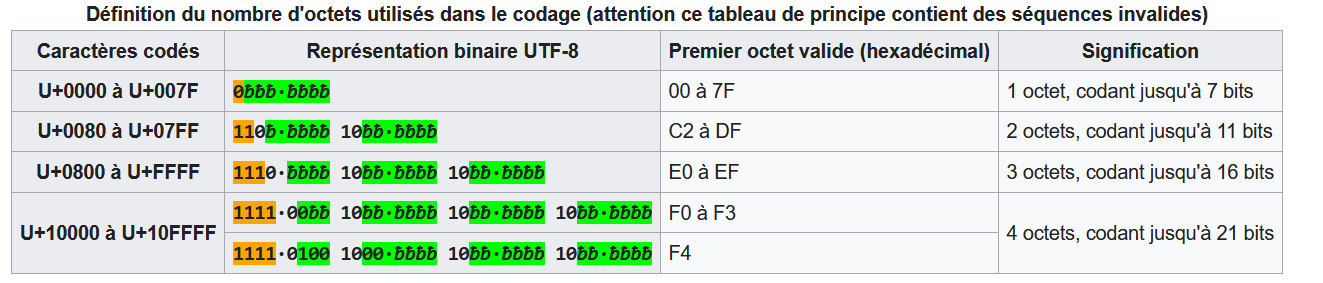
\includegraphics[width=1.0\textwidth]{utf8.png}
\caption{Le codage de l'UTF-8 selon wikipedia}
\label{fig:utf8}
\end{figure}

\end{document}
